%! Author = charon
%! Date = 6/4/24

\section{Analyse der Fuzzer Performance}\label{sec:analyse-der-performance}
In diesem Kapitel wird die Performance von \gls{afl}Net, Pulsar und boofuzz analysiert.
Der Begriff Performance ist jedoch sehr vielseitig zu interpretieren und wird in dieser Arbeit unter den Gesichtspunkten
Effektivität, Geschwindigkeit und Reproduzierbarkeit bewertet.\newline
Die Effektivität eines Fuzzers wird anhand der Anzahl der gefundenen Bugs gemessen.
Die Geschwindigkeit eines Fuzzers wird anhand der Anzahl der generierten Eingaben pro Sekunde gemessen.
Die Reproduzierbarkeit eines Fuzzers wird anhand der Anzahl der reproduzierten Bugs gemessen.
Zur Analyse der Performance werden die Fuzzer \gls{afl}Net, Pulsar und boofuzz verwendet.\newline\newline
Zur Analyse der Effektivität wurden drei Schwachstellen im \gls{mqtt} Protokoll implementiert.
Die Schwachstellen belaufen sich auf drei Buffer Overflows und Seiteneffekte von der Aufhebung von Sanity-Checks beim
Empfangen einer Publish-Nachricht.
Diese implementierten Schwachstellen wurden an verschiedenen Stellen im \gls{mqtt} Broker Mosquitto eingefügt, sodass
auch eine Bewertung der Komplexität der gefundenen Schwachstelle erfolgen kann.
Die einfachste Schwachstelle ist ein Buffer Overflow in der Funktion \texttt{mqtt\_handle\_connect} (Listing~\ref{lst:handle-connect}) und wird genau dann
getriggert, wenn ein Client eine Verbindung zum Broker aufbaut und der Client im Payload über eine \texttt{will}-Nachricht
verfügt.
Die mittlere Schwachstelle ist ein Integer Overflow in der Funktion \texttt{mqtt\_handle\_publish} (Listing~\ref{lst:handle-publish}) und wird getriggert,
wenn ein Client eine Nachricht an den Broker sendet und die Nachricht eine bestimmte Länge überschreitet.
Diese Schwachstelle kann nur getriggert werden, wenn ein Client \texttt{C1} ein Topic mit einer Nachricht veröffentlicht hat und ein
zweiter Client \texttt{C2} dieses Topic abonniert hat.
Nur in diesem Fall wird auch die von \texttt{C1} veröffentlichte Nachricht an \texttt{C2} weitergeleitet und auch vom Broker verarbeitet.
Die komplexeste Schwachstelle ist ein Memory Leak in der Funktion \texttt{mqtt\_handle\_subscribe} (Listing~\ref{lst:handle-subscribe}) und wird getriggert,
wenn ein Client ein Topic abonniert und der Broker die Abonnement-Nachricht verarbeitet.
%! Author = chaorn
%! Date = 13.08.24

\subsection{Fuzzing mit AFLNet}\label{subsec:aflnet}
Das folgende Kapitel beschreibt das Aufsetzen der Testumgebung und die darin durchgeführten Experimente mit dem Fuzzing-Tool
\gls{afl}Net.
\subsubsection{Setup}
Da \gls{afl}Net legacy Software ist, wird es nicht mehr aktiv weiterentwickelt und an neue Frameworks und Bibliotheken
angepasst.
Zum Kompilieren von \gls{afl}Net wird hierzu ein angepasstes Dockerfile~\cite{aflnet-dockerfile} verwendet.
Dieses angepasste Dockerfile enthält alle notwendigen Abhängigkeiten, um \gls{afl}Net zu kompilieren.
Hierzu zählen die Abhängigkeiten \texttt{llvm} und \texttt{clang} in der Version 11.
\texttt{llvm} wird benötigt, um den \gls{afl} Compiler \texttt{afl-clang-fast} zu kompilieren.
Dieser wird für optimierte Instrumentierung des Codes des \gls{zup} verwendet und bezweckt somit höhere Ausführgeschwindigkeiten
während der Fuzzing Kampagne.
Für die erfolgreiche Verwendung des Compilers \texttt{afl-clang-fast} musste für die Kompatibilität mit einer neueren
Ubuntu-Version ein Patch~\cite{llvm-patch} für das Kompilieren des Compilers geschrieben werden.\newline
Das \gls{zup} Mosquitto wird ebenfalls in einem Docker Container kompiliert.
Hierzu wird der Compiler \texttt{afl-clang-fast} verwendet.
Die Instrumentierung des Codes erfolgt durch das Flag \texttt{-fsanitize=address}.
Dieses Flag aktiviert \textit{address sanitization} und ermöglicht es, dass \gls{afl}Net die Speicherzugriffe des \gls{zup}
überwachen kann und somit Buffer Overflows und Memory Leaks erkennt.
Zum Starten des Mosquitto-Bianrys wurde außerdem eine \textit{preloaded-library}~\cite{mqtt-preload} verwendet, die alle Ausgaben des \gls{zup}
aus den Kanälen \texttt{stdout} und \texttt{stderr} in eine log-Datei \texttt{mqtt-aflnet\_stdout.log} weiterleitet.
Diese Log-Datei wird benötigt, um die Ausgaben des \gls{zup} zu analysieren und somit die Effektivität der generierten
Testcases zu bewerten. \newline
Die Testcases wurden mithilfe eines Python-Skripts~\cite{aflnet-generate-test} generiert.
Die Struktur wurde hierzu aus bereits existierenden Nachrichten einer \gls{pcap}-Datei mithilfe von Wireshark extrahiert.
Anhand der Struktur der Bytes wurden die Nachrichten in ein Format umgewandelt, das von \gls{afl}Net verstanden wird.
Die in Kapitel~\ref{subsec:mosquitto-mqtt} beschriebene Struktur einer \gls{mqtt} Nachricht wurde dazu verwendet.
In dieser Nachricht kann der Fixed-Header den Bytes \texttt{0x10, 0x30, 0x82, 0xA2, 0xC0} und \texttt{0xE0} entsprechen.
Diese stehen für die verschiedenen Anfragen \texttt{CONNECT, PUBLISH, SUBSCRIBE, UNSUBSCRIBE, PINGREQ} und \texttt{DISCONNECT}.
Die Variable Header und Payload wurden zufällig generiert und in die Testcases eingefügt.
Die Testcases wurden in einem Verzeichnis \texttt{aflnet\_in/} abgelegt und von \gls{afl}Net als Eingabe verwendet.
Damit möglichst viele States beim Ausführen des \gls{zup} erreicht werden, wurden ebenfalls ungültige Pakete generiert.
Sie dienen \gls{afl}Net dazu, unerwartete Zustände des \gls{zup} zu erreichen und somit unerwartete Bugs zu finden.
Des Weiteren wurden Nachrichtensequenzen generiert, die den Zustand des \gls{zup} verändern.
Hierzu wurden alle Nachrichten, die der \gls{zup} verarbeiten kann, in einer Sequenz aneinandergereiht.
Diese Sequenzen wurden ebenfalls in das Verzeichnis \texttt{aflnet\_in/} abgelegt und von \gls{afl}Net als Eingabe verwendet.
\subsubsection{Analyse der Effektivität gesendeter Pakete}
Die Fuzzing-Kampagne wurde über einen Zeitraum von 48 Stunden durchgeführt.
Zur Analyse der Effektivität der gesendeten Pakete wurde eine preload bibliothek verwendet, die die Ausgaben des \gls{zup}
der Kanäle \texttt{sdtout} und \texttt{stderr} in eine Log-Datei \texttt{mqtt-aflnet\_stdout.log} umleitet.
Mit den folgenden Experimenten und Auswertungen soll ein Teil der Forschungsfrage \textit{Q1}~\ref{researc-questions}
beantwortet werden.
Nun wird analysiert, wie effektiv die generierten Nachrichten des \gls{afl}Net-Fuzzers sind.\newline
Diese Log-Datei wurde auf die Häufigkeit der Ausgaben von erfolgreichen und fehlgeschlagenen Verbindungsaufbauten analysiert.
\begin{figure}[H]
    \centering
    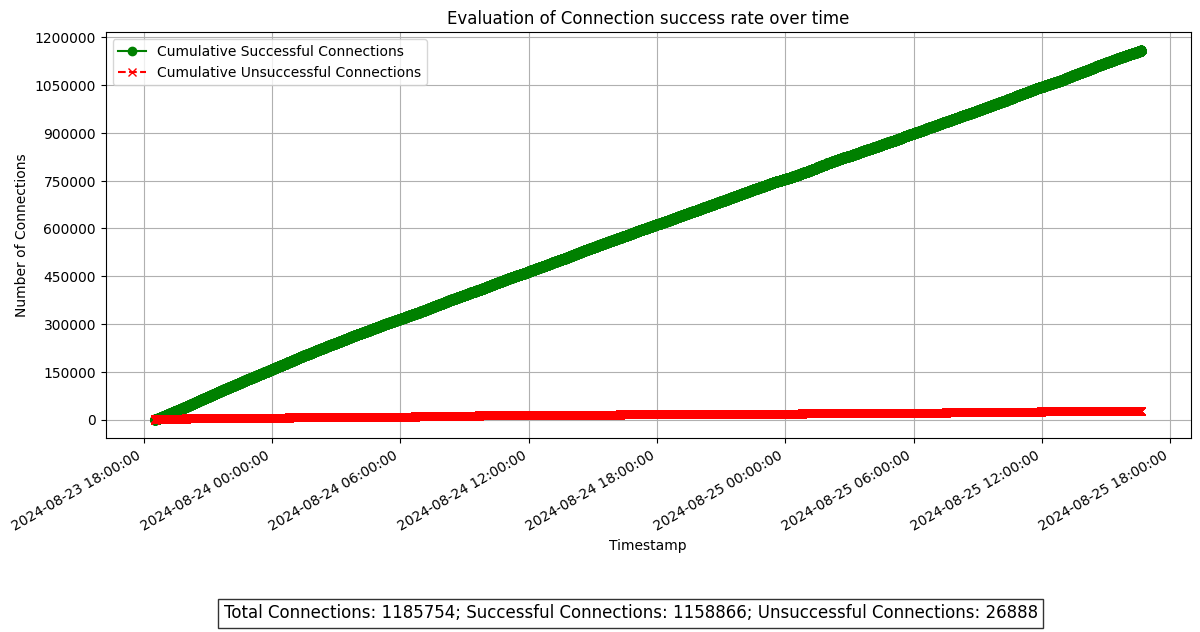
\includegraphics[width=\textwidth]{img/connection_evaluation_aflnet}
    \caption[Diagram zur Auswertung erfolgreicher Verbindungsaufbauten mit dem \gls{mqtt}-Protokoll]{Evaluation der Verbindungsaufbauten des \gls{zup} Mosquitto. Die Log-Datei \texttt{mqtt-aflnet\_stdout.log}
    wurde auf die Häufigkeit der Ausgaben von erfolgreichen und fehlgeschlagenen Verbindungsaufbauten analysiert.}
    \label{fig:mqtt-aflnet_stdout}
\end{figure}
\noindent Die grüne Linie (siehe Abb.~\ref{fig:mqtt-aflnet_stdout}) repräsentiert die Anzahl der erfolgreichen Verbindungen im Laufe der Zeit.
Die Linie steigt linear an und erreicht gegen Ende der Kampagne eine Gesamtzahl von 1.158.866 erfolgreichen Verbindungen.
Dies deutet darauf hin, dass das getestete System eine sehr hohe Erfolgsrate bei Verbindungsversuchen aufweist.
Die lineare Zunahme zeigt, dass die Rate der erfolgreichen Verbindungen konstant hoch geblieben ist, ohne signifikante
Einbrüche oder Schwankungen.
Die rote Linie (siehe Abb.~\ref{fig:mqtt-aflnet_stdout}) zeigt die Anzahl der erfolglosen Verbindungen an.
Diese bleibt über den gesamten Zeitraum sehr niedrig und erreicht gegen Ende der Kampagne etwa 26.888 erfolglose Verbindungen.
Dies entspricht einer Erfolgsrate von über \SI{97}{\percent} und einer Fehlerrate von ca. $\sim \SI{2.32}{\percent}$
in denen \gls{afl}Net keine erfolgreichen Verbindungsaufbauten mit dem \gls{mqtt}-Broker über das \gls{mqtt}-Protokoll
entstanden sind.
Der minimale Anstieg im Vergleich zu den erfolgreichen Verbindungen weist darauf hin, dass die Mehrheit der Verbindungen
erfolgreich war.
Bei der Analyse der Fehleranfälligkeit von nicht validen Nachrichten wurde festgestellt, dass am Anfang der Fuzzing-Kampagne
viele Fehlermeldungen auftraten.
Mit der Zeit wurden jedoch weniger Fehlermeldungen generiert, da die State Machine des \gls{zup} erlernt wurde und somit
vermehrt valide Nachrichten generiert wurden.
\begin{figure}[H]
    \centering
    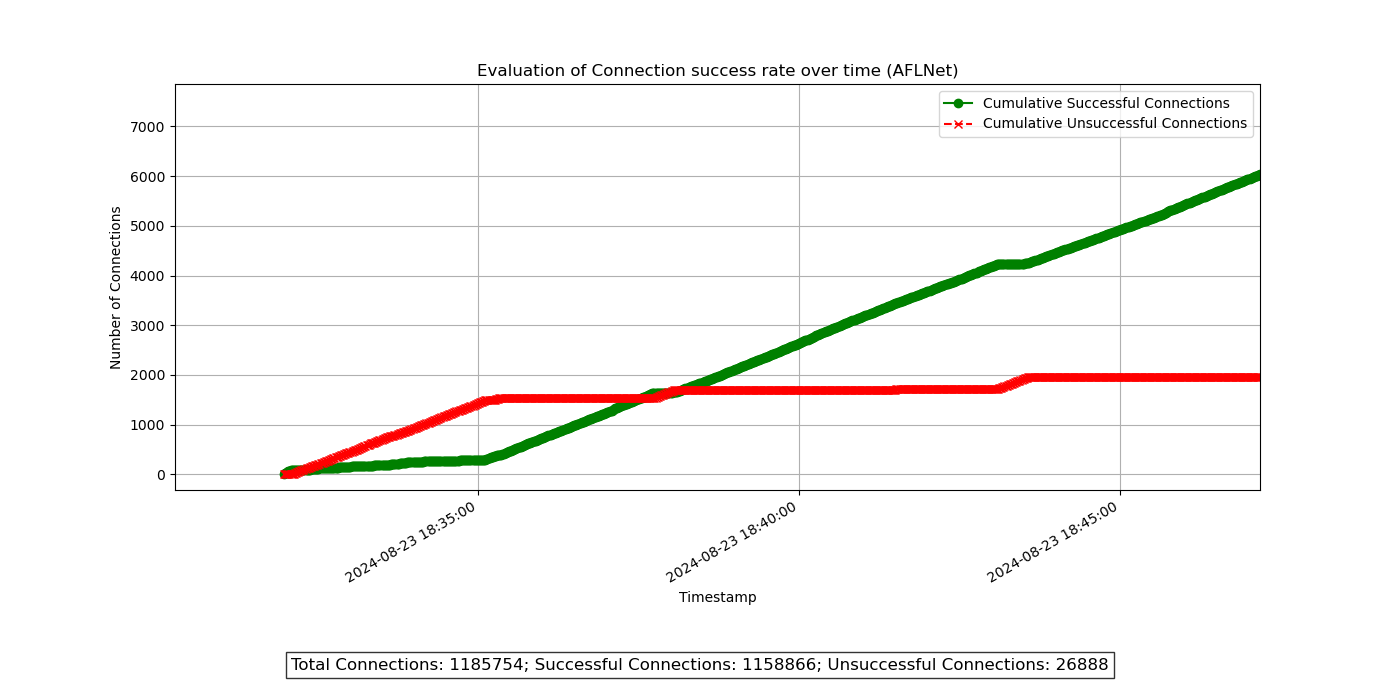
\includegraphics[width=\textwidth]{img/connection_evaluation_aflnet_beginning}
    \caption[Diagram zur Auswertung erfolgreicher Verbindungsaufbauten mit dem \gls{mqtt}-Protokoll zu Beginn der Fuzzing Kampagne]{
        Dieses Diagramm zeigt eine vergrößerte Ansicht der ersten
        10 Minuten der Fuzzing-Kampagne aus Abbildung~\ref{fig:mqtt-aflnet_stdout} mit \gls{afl}Net zur Veranschaulichung der Fehleranfälligkeit zu Beginn der Fuzzing-Kampagne.
        Aus dem Diagramm geht hervor, dass zu Beginn der Kampagne viele erfolglose Verbindungen mit dem \gls{zup} generiert
        wurden, die jedoch im Laufe der Zeit abnahmen.
    }
    \label{fig:mqtt-aflnet_stdout_beginning}
\end{figure}
\noindent Das Diagramm (siehe Abb.~\ref{fig:mqtt-aflnet_stdout_beginning}) zeigt deutlich, dass die Lernphase der State-Machine
zu Beginn der Fuzzing-Kampagne von Bedeutung ist.
Die hohe Anzahl von erfolglosen Verbindungen in der Anfangsphase deutet darauf hin, dass die anfänglichen Eingaben von 
\gls{afl}Net nicht korrekt auf das getestete System abgestimmt waren. 
Erst nach einer gewissen Zeit, in der die State-Machine genügend Informationen gesammelt hat, um die Struktur des Protokolls 
besser zu verstehen, beginnt die Anzahl der erfolgreichen Verbindungen anzusteigen.
Dieses Verhalten zeigt, dass das System Zeit benötigt, um die richtigen Eingabenmuster zu lernen. 
Dieser Lernprozess führt zu einer sukzessiven Verbesserung der Qualität der generierten Eingaben und damit zu einer 
steigenden Erfolgsrate bei den Verbindungen.
\subsubsection{Analyse der Geschwindigkeit}
\begin{figure}[H]
    \centering
    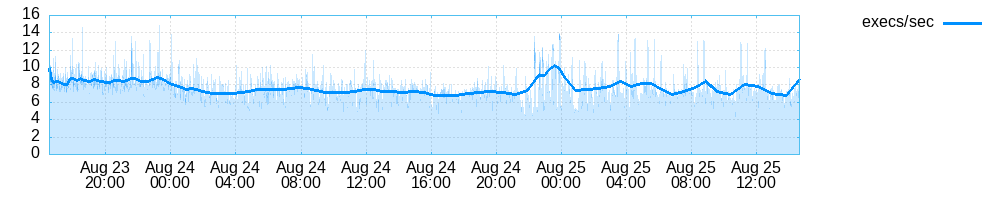
\includegraphics[width=\textwidth]{img/exec_speed}
    \caption[Diagramm zur Veranschaulichung der Ausführungsgeschwindigkeit von AFLNet während der Fuzzing-Kampagne]{Diese Abbildung zeigt die Ausführgeschwindigkeit von \gls{afl}Net.
    Es wird die Anzahl der Nachrichtensequenzen pro Sekunde (y-Achse), die an das \gls{zup} während des Zeitrahmens der
    Kampagne (x-Achse) gesendet wurden, veranschaulicht.}
    \label{fig:aflnet_execs}
\end{figure}
\noindent Die Ausführungsrate ist eine Metrik, um den Fortschritt und die Effektivität einer Fuzzing-Kampagne zu bewerten.
Eine hohe und stabile Ausführungsrate deutet auf einen effizienten Fuzzing-Prozess hin, während Schwankungen oder ein
Rückgang auf potenzielle Engpässe oder Herausforderungen während der Kampagne hinweisen können.\newline
Die Ausführungsrate liegt im Durchschnitt zwischen 6 und 10 execs/sec und zeigt eine gewisse Variabilität, wie durch die
Spitzen und Täler in der hellblauen Schattierung dargestellt.
Anzumerken ist, dass das \gls{zup} mit einem AddressSanitizer kompiliert wurde, was die Ausführungsgeschwindigkeit
beim Fuzzing verlangsamt.
Das resultiert aus dem zusätzlichen Speicher, welchen bei Start des Programms allokiert wird, um die Speicherzugriffe
zu überwachen.
Zu Beginn der Kampagne gibt es einen kurzen Zeitraum mit erhöhter Variabilität, bevor sich die Ausführungsrate stabilisiert.
Im weiteren Verlauf der Kampagne ist eine leichte Abnahme der Ausführungsrate zu beobachten, gefolgt von einer leichten
Erholung gegen Ende der Kampagne.
Die Kurve zeigt während der gesamten Kampagne eine relativ konstante Ausführungsrate mit periodischen Schwankungen.
Diese Schwankungen können auf mehrere Faktoren zurückzuführen sein, darunter:
\begin{itemize}
    \item Komplexität der zu testenden Eingaben: Komplexere Testfälle können mehr Zeit in Anspruch nehmen, was die Ausführungsrate verringert.
    \item Systemressourcen: Veränderungen in der Verfügbarkeit von Systemressourcen (z.B.\ CPU, Speicher) können ebenfalls die Ausführungsrate beeinflussen.
    \item Optimierungen oder Veränderungen im Fuzzing-Prozess: Wenn das Fuzzing-Tool neue Pfade oder besonders anspruchsvolle Testfälle entdeckt, kann dies die Rate der durchgeführten Tests vorübergehend senken.
\end{itemize}
\noindent Ein leichtes Absinken der Ausführungsrate zwischen dem 24. August, 12:00 Uhr, und dem 25. August, 00:00 Uhr, ist bemerkenswert.
Dies könnte darauf hindeuten, dass in dieser Phase anspruchsvollere Testfälle bearbeitet wurden oder dass die Systemressourcen
temporär begrenzt waren.
Die anschließende Erholung der Ausführungsrate könnte durch die Verarbeitung weniger komplexer Testfälle oder eine bessere
Ausnutzung der Systemressourcen erklärt werden.
Die insgesamt stabile Ausführungsrate über den Zeitraum von 48 Stunden deutet auf einen stabilen Fuzzing-Prozess hin.
Die beobachteten Schwankungen sind im Rahmen dessen, was bei längeren Fuzzing-Kampagnen zu erwarten ist, und weisen auf
die normale Dynamik im Fuzzing-Prozess hin, wenn unterschiedliche Testfälle mit variierender Komplexität ausgeführt werden.
Die leichte Abnahme der Ausführungsrate gegen Ende der Kampagne könnte als Hinweis darauf gewertet werden, dass das Tool
zunehmend anspruchsvollere Testfälle oder Pfade bearbeitet hat.
Außerdem anzumerken ist, dass eine Ausführung von \gls{afl}Net dem Starten des \gls{zup}, dem anschließenden
Senden einer Nachricht aus dem Fuzzing Corpus und dem Beenden des \gls{zup} entspricht.
Dem zu entnehmen ist, dass bei Komplexen \gls{iot} Protokollen die Ausführungsrate geringer ausfallen kann, da die
Initialisierung des \gls{zup} und das Senden einer Nachricht mehr Zeit in Anspruch nehmen kann.
\begin{figure}[H]
    \centering
    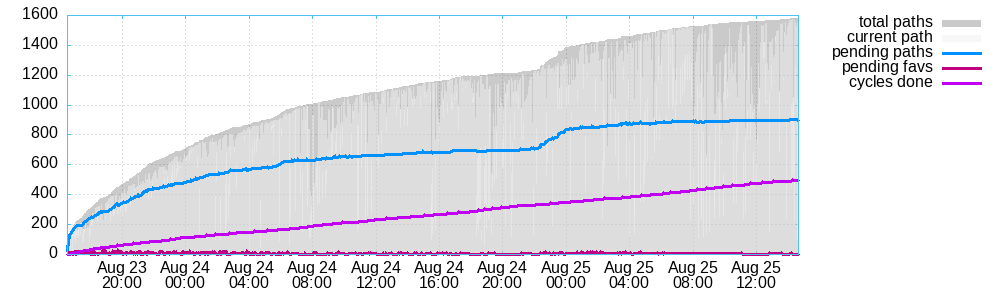
\includegraphics[width=\textwidth]{img/high_freq}
    \caption[]{Das Diagramm veranschaulicht das Eingabegenerierungsverhalten von \gls{afl}Net während der Fuzzing-Kampagne.
    Die y-Achse gibt einen numerischen Wert an, welcher im Kontext zu den abgebildeten Graphen zu betrachten ist.}
    \label{fig:aflnet_speed}
\end{figure}
\noindent Das gezeigte Diagramm veranschaulicht den Verlauf einer 48-stündigen Fuzzing-Kampagne mit dem \gls{afl}Net-Tool, wobei
verschiedene Metriken im Zusammenhang mit der Testabdeckung und dem Fortschritt des Fuzzing-Prozesses dargestellt werden.
Im Folgenden werden die verschiedenen Kurven analysiert und ihre Bedeutung in Bezug auf die Kampagne erläutert.\newline\newline
Die graue Fläche (siehe Abb.~\ref{fig:aflnet_speed}) zeigt die Gesamtanzahl der explorierten Pfade während der Kampagne.
Diese Zahl steigt kontinuierlich an und erreicht gegen Ende der Kampagne über 1400 Pfade.
Der gleichmäßige Anstieg deutet darauf hin, dass der Fuzzer während der gesamten Kampagne effektiv neue Pfade
identifizieren konnte.
Interessanterweise gibt es Phasen, in denen der Anstieg steiler ist, was auf eine besonders hohe Entdeckungsrate neuer
Pfade in diesen Perioden hinweist.\newline
Die hellblaue Linie (siehe Abb.~\ref{fig:aflnet_speed}) repräsentiert den aktuell im Test befindlichen Pfad.
Diese Kurve zeigt, wie das Fuzzing-Tool ständig neue Pfade auswählt und testet.
Die Linie verläuft relativ flach, was darauf hinweist, dass das Fuzzing-Tool regelmäßig zwischen den Pfaden wechselt und
keiner besonders lange untersucht wird.
Diese regelmäßige Bewegung zwischen den Pfaden kann auf eine gleichmäßige Verteilung der Testressourcen hinweisen.\newline
Die Anzahl der noch zu testenden Pfade (blau, siehe Abb.~\ref{fig:aflnet_speed}) zeigt einen Anstieg, der während der gesamten Kampagne
andauert und gegen Ende der 48 Stunden fast 600 erreicht.
Dies bedeutet, dass das Fuzzing-Tool konstant neue Pfade entdeckt hat, die es noch zu testen gilt.
Der kontinuierliche Anstieg zeigt, dass das System immer neue potenziell interessante Zustände produziert, die eine
weitere Untersuchung erfordern.\newline
Die lila Kurve (siehe Abb.~\ref{fig:aflnet_speed}) stellt die favorisierten Pfade dar, die noch nicht getestet wurden.
Diese Zahl steigt ebenfalls stetig an, jedoch langsamer als die \enquote{pending paths}(siehe Abb.~\ref{fig:aflnet_speed}).
Dies deutet darauf hin, dass das Fuzzing-Tool bestimmte Pfade als besonders wichtig erachtet und diese bevorzugt behandelt,
obwohl noch viele andere Pfade auf ihre Untersuchung warten.
Diese Priorisierung kann dazu beitragen, dass besonders interessante oder sicherheitsrelevante Pfade frühzeitig getestet werden.
Die magentafarbene Kurve (siehe Abb.~\ref{fig:aflnet_speed}) zeigt die Anzahl der abgeschlossenen Testzyklen.
Diese steigt über die Zeit an, was die Fortschritte im Fuzzing-Prozess darstellt.
Ein Zyklus umfasst die vollständige Durcharbeitung des aktuellen Satzes von Testfällen.
Der Anstieg zeigt, dass das Fuzzing-Tool kontinuierlich neue Zyklen durchläuft, was auf eine fortlaufende und systematische
Prüfung der Pfade hinweist.
\begin{figure}[H]
    \centering
    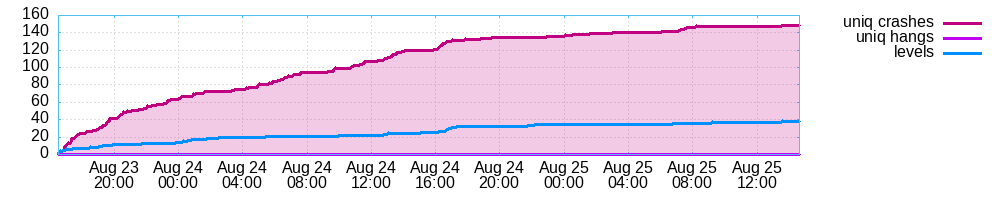
\includegraphics[width=\textwidth]{img/low_freq}
    \caption[Grafik zur Veranschaulichung der Gefundenen Bugs mit AFLNet]{Diese Abbildung zeigt die Anzahl der gefundenen
    Bugs (auf der y-Achse) von \gls{afl}Net in Relation zur vergangenen Zeit (x-Achse).}
    \label{fig:aflnet_bugs}
\end{figure}
\noindent Die Anzahl der einzigartigen Abstürze (pink siehe Abb.~\ref{fig:aflnet_bugs}) zeigt einen kontinuierlichen Anstieg über den gesamten Kampagnenzeitraum.
Besonders auffällig ist der steile Anstieg zu Beginn der Kampagne, gefolgt von einem moderateren Anstieg, der sich über
den Rest der Kampagne hinweg fortsetzt.
Dies deutet darauf hin, dass in den ersten Stunden der Kampagne eine größere Anzahl an Abstürzen entdeckt wurde, was
typisch für Fuzzing-Kampagnen ist, bei denen anfänglich viele triviale Schwachstellen gefunden werden.
Im weiteren Verlauf der Kampagne werden dann weniger neue Abstürze entdeckt, was darauf hinweist, dass das System bereits
viele der simpleren potenziellen Schwachstellen aufgedeckt hat.
Die Anzahl der einzigartigen Hänger (magenta, siehe Abb.~\ref{fig:aflnet_bugs}) bleibt über den gesamten Kampagnenzeitraum stabil bei null.
Dies könnte darauf hindeuten, dass entweder keine Hänger im getesteten System aufgetreten sind oder dass das verwendete
Fuzzing-Setup nicht in der Lage war, solche Zustände effektiv zu identifizieren.
Die Levels-Kurve (blau, siehe Abb.~\ref{fig:aflnet_bugs}) zeigt nur einen leichten Anstieg in den ersten Stunden der Kampagne und bleibt danach weitgehend konstant.
Dies könnte darauf hinweisen, dass nur wenige neue Code-Pfade (Levels) während des Fuzzings entdeckt wurden, was
möglicherweise auf die Komplexität des Zielsystems oder auf die Grenzen der verwendeten Mutationsstrategien hinweist.
Die Fuzzing-Kampagne mit \gls{afl}Net war erfolgreich darin, eine beträchtliche Anzahl einzigartiger Abstürze zu entdecken,
insbesondere in den ersten Stunden des Fuzzings.
Der Mangel an identifizierten Hängern und der begrenzte Anstieg an Levels könnte jedoch darauf hinweisen, dass entweder
das Zielsystem keine anfälligen Hängerzustände aufweist oder dass das Fuzzing-Setup verbessert werden könnte, um diese
Art von Fehlern besser zu identifizieren.
\subsubsection{Analyse der gefundenen Bugs}\label{subsubsec:bugs}
Die gefundenen Bugs nach der 48-stündigen Fuzzing-Kampagne belaufen sich auf 151 Bugs (siehe Abb.~\ref{fig:aflnet_bugs}).
Hierzu wurden alle Abstürze mithilfe von Bash-Skripts dokumentiert~\cite{crash-extraction-script} und analysiert~\cite{analyse-crashes-script}.
Bei allen gefundenen Bugs handelt es sich um \textit{Segmentation Faults} und konnten in vier Kategorien eingeteilt werden:
\begin{enumerate}
    \item Absturz durch Buffer Overflow in der Funktion \texttt{packet\_\_write\_bytes} \\in \texttt{lib\/packet\_datatypes.c}
    \item Absturz durch Buffer Overflow in der Funktion \texttt{packet\_\_write\_bytes} \\in \texttt{lib\/packet\_datatypes.c}
    mit einer \gls{qos}-Nachricht
    \item Absturz durch Buffer Overflow in der Funktion \texttt{packet\_\_write\_bytes} \\in \texttt{lib\/packet\_datatypes.c}
    mit einer \gls{qos}-Nachricht und einem subscriber
    \item Absturz durch Buffer Overflow in der Funktion \texttt{handle\_\_publish} in \\\texttt{src\/handle\_publish.c}
\end{enumerate}
Die Abstürze der vierten Kategorie sind auf die eigene Implementierung eines Buffer Overflows zurückzuführen.
Dieser Buffer Overflow wird getriggert, da die Sanity-Checks (~\ref{lst:mqtt-sainity-checks}) in der Funktion \texttt{handle\_\_publish} auskommentiert
wurden.
Diese Sanity-Checks überprüfen, ob die Länge der Nachricht, die an den Broker gesendet wird, korrekt ist.
Der Fehler tritt nach dem auskommentierten Sanity-Check auf, wenn darauf geprüft wird, ob die Nachricht, die gesendet
werden soll bereits existiert.
Hierzu soll die gesendete Nachricht -- mit einer bereits vorhandenen Nachricht-ID -- mit der bereits zwischengespeicherten
Nachricht verglichen werden.
Diese Nachricht mit der gleichen ID ist jedoch größer als die bereits zwischengespeicherte Nachricht und führt bei dem
Vergleich mit \texttt{memcmp} zum Absturz des \gls{zup}.
\newline
Die anderen drei Kategorien sind gleichen Ursprungs.
Hier handelt es sich um einen Buffer Overflow in der Funktion \texttt{packet\_\_write\_bytes} in der Datei \\
\texttt{lib\/packet\_datatypes.c}.
Diese Schwachstelle wird bei dem Senden der Nachricht an ein Topic ausgelöst.
Hierbei werden Nachrichten vom Broker empfangen und das Topic weitergeleitet.
Wenn Subscriber auf das Topic warten, wird die Nachricht an die Subscriber mittels des Syscalls \texttt{memcpy} weitergeleitet.
\newline
Die Gesamterscheinungen der Bugs belaufen sich auf 151 Bugs, von denen 105 dem Fehler in der Funktion
\texttt{handle\_\_publish} entsprechen.
Die restlichen 46 Bugs entstammen den Buffer Overflows in der Funktion \texttt{packet\_\_write\_bytes}.
\newline
Die gefundenen Bugs wurden mithilfe des Tools \texttt{aflnet-replay} reproduziert und auf ihre Validität überprüft.
Sie zeigten jedoch keine Wirkung auf den Broker ohne manuell implementierte Schwachstellen.\newline\newline
Zusammenfassend lässt sich sagen, dass \gls{afl}Net nur zwei Schwachstellen im Broker Mosquitto gefunden hat, von denen
beide von der Implementierung der Sanity-Checks abhängen.
Wichtig anzumerken ist, dass \gls{afl}Net einen Absturz genau dann als einzigartig betrachtet, wenn die an das \gls{zup}
übergebene Nachricht einen neuen Pfad im Code des \gls{zup} erreicht.
Die Stelle, an der das \gls{zup} zum Absturz gebracht wird, ist für \gls{afl}Net nicht ausschlaggebend.
%! Author = chaorn
%! Date = 13.08.24

\subsection{Fuzzing mit boofuzz}\label{subsec:boofuzz}
In dem folgenden Kapitel wird das Aufsetzen der Testumgebung und die darin durchgeführten Experimente mit dem Fuzzing-Tool
boofuzz beschrieben.
\subsubsection{Setup}
Zur Entwicklung einer Fuzzing-Kampagne mit boofuzz sind mehrere Schritte erforderlich.
Zunächst muss das Zielsystem identifiziert und analysiert werden, um die relevanten Protokollspezifikationen und
Kommunikationsmuster zu verstehen.
Darauf aufbauend werden die Testfälle definiert, die die verschiedenen Protokollfelder und Eingabeparameter abdecken sollen.
Die Testfälle werden in boofuzz als \textit{Fuzz-Template} definiert, das die Struktur und den Inhalt der zu füllenden
Nachrichten beschreibt.
Das Fuzz-Template besteht aus einer Reihe von Feldern, die die verschiedenen Teile der Nachricht repräsentieren, wie z.B.\ den
Fixed Header, den Variable Header und den Payload bei \gls{mqtt}-Nachrichten.
Jedes Feld kann verschiedene Eigenschaften wie den Typ, die Länge und den Wertebereich der Eingabe enthalten.
In dem Fall der \gls{mqtt}-Nachrichten können die Felder z.B.\ den Steuerpakettyp, die QoS-Ebene und den Topic-Namen,
wie in Kapitel~\ref{subsec:mosquitto-mqtt} beschrieben, repräsentieren.
Hierbei ist es wichtig, die Protokollspezifikationen und die erwarteten Eingabewerte zu berücksichtigen, um realistische
Testfälle zu erstellen.
Nachdem die Testfälle definiert sind, wird eine Fuzzing-Kampagne gestartet, bei der boofuzz automatisch eine Vielzahl
von zufälligen oder systematischen Eingaben generiert und an das Zielsystem sendet.
Während des Fuzzings kann boofuzz den Zustand des Zielsystems überwachen und auf unerwartete Ereignisse wie Abstürze oder
Fehler reagieren.
Dieser Schritt ist jedoch nicht standardmäßig eingebaut und muss vom Benutzer implementiert werden.
Die Implementierung der Reaktion auf unerwartete Ereignisse kann z.B.\ das Neustarten des Zielsystems, das Anpassen der
Fuzzing-Strategie oder das Protokollieren von Fehlern umfassen und erfolgt über ein in boofuzz implementiertes Interface.
Dieses Interface beinhaltet die Monitor-Klassen \texttt{ProcessMonitor, NetworkMonitor} und \texttt{CallbackMonitor}.
Die \texttt{ProcessMonitor}-Klasse überwacht den Zustand des Zielsystems, indem sie den Prozessstatus überwacht und auf
Abstürze oder Fehler reagiert.
Dieser Monitor wurde zum Beispiel in der Analyse des \gls{mqtt}-Brokers Mosquitto verwendet, um auf Abstürze des Brokers
zu reagieren und die in den Abstürzen enthaltene debug-Informationen abzugreifen und zu speichern.
\newline\newline
Eine in dieser Arbeit verwendete Kernkomponente von boofuzz ist die Option ein Feld als \texttt{fuzzable} zu definieren.
Ein \texttt{fuzzable} Feld ist ein Feld, das zufällig generierte Eingaben erhalten darf und somit für das Fuzzing relevant ist.
Mit dieser Option können Testfälle erstellt werden, die systematisch verschiedene Eingaben in bestimmte Felder einfügen,
um präzisere und effektivere Fuzzing-Kampagnen durchzuführen.
Die \texttt{fuzzable}-Option ermöglicht es, die Eingaben gezielt zu steuern und bestimmte Protokollfelder oder Eingabeparameter
zu testen, um potenzielle Schwachstellen zu identifizieren.
Gerade im Fall von \gls{mqtt}-Nachrichten ist es wichtig, die verschiedenen Felder wie den Fixed Header, den Variable Header
und den Payload systematisch zu füllen.
\newline\newline
Für das Entwickeln einer Fuzzing-Kampagne wurden im Rahmen dieser Arbeit zwei Module entwickelt:
\begin{itemize}
    \item boo-fuzzer-mqtt
    \item boo-fuzzer-mqtt-efficient
\end{itemize}
Das Modul \texttt{boo-fuzzer-mqtt} enthält die Implementierung einer Fuzzing-Kampagne für den \gls{mqtt}-Broker weitestgehend
ohne statisch definierte Felder.
Alle Teilaspekte eines Pakets als fuzzable zu definieren kann in vielen Fällen Sinn machen, um die gesamte Struktur eines
Netzwerkpakets zu testen.
Hierzu können alle individuellen Teile einer \gls{mqtt}-Nachricht auf richtige Verarbeitung getestet werden.\newline
Das Modul \texttt{boo-fuzzer-mqtt-efficient} hingegen definiert statische Felder für den Fixed Header, den Variable Header
und das Topic.
Das Topic wird hierbei als \texttt{fuzzing/topic} fest vordefiniert und gepublisht, sodass jede einhergehende Client-Verbindung
bereits ein Topic zur Verfügung hat.
Das hat zur Folge, dass die Wahrscheinlichkeit, dass ein gültiges Paket generiert wird, signifikant erhöht wird.
Für das Starten einer Fuzzing-Kampagne mit boofuzz sind folgende Schritte notwendig:
\begin{itemize}
    \item Installation von boofuzz und den erforderlichen Abhängigkeiten
    \item Definition der Testfälle und Fuzzing-Strategien
    \item Starten der Fuzzing-Kampagne und Überwachung des Zielsystems
    \item Analyse der Ergebnisse und Identifizierung von Schwachstellen
\end{itemize}
Zusätzlich kommt hinzu, dass bei der effizienten Lösung der Broker bereits in einen preparierten Zustand versetzt wird,
sodass weniger Overhead bei der initialen Fuzzingstrategie entsteht.
Außerdem muss ein Monitor für das \gls{zup} definiert werden, sodass auch das automatische Starten, Neustarten und Beenden
des Zielsystems möglich ist und bei Abstürzen die entsprechenden Informationen des Absturzes sammeln zu können.
\subsubsection{Analyse der Effektivität gesendeter Pakete}
In der Untersuchung von \gls{mqtt}-Brokern mittels Fuzzing ist es entscheidend, die Wahrscheinlichkeit zu verstehen, mit der
ein zufällig generiertes Paket tatsächlich gültig ist.
Diese Wahrscheinlichkeit hängt stark davon ab, welche Teile des \gls{mqtt}-Pakets zufällig generiert werden und welche festgelegt
(d.h.\ nicht gefuzzt) sind.
In diesem Abschnitt wird die Berechnung dieser Wahrscheinlichkeit detailliert beschrieben, sowohl für den Fall, dass alle
Teile des Pakets gefuzzt werden, als auch für den Fall, dass bestimmte Teile, wie der Fixed Header und der Variable Header,
festgesetzt sind.
Dieser Teil adressiert die Forschungsfrage \textit{Q1}~\ref{researc-questions} und beschäftigt sich mit der Auswertung
und Analyse der Effektivität und Erfolgsrate der generierten Eingaben mit boofuzz.\newline\newline
\noindent Ein \gls{mqtt}-Paket besteht aus mehreren wesentlichen Teilen:
\begin{itemize}
    \item Fixed Header: Enthält den Steuerpakettyp (z.B.\ \texttt{PUBLISH, SUBSCRIBE}) und Flags sowie die verbleibende Länge des Pakets.
    \item Variable Header: Enthält je nach Steuerpakettyp spezifische Informationen wie z.B.\ Paket-IDs, QoS-Level oder den Namen des Topics.
    \item Payload: Enthält die tatsächlichen Daten, die gesendet werden (z.B.\ die Nachricht im \texttt{PUBLISH}-Paket)
    oder eine Liste von Topic-Filtern im \texttt{SUBSCRIBE}-Paket.
\end{itemize}
\begin{figure}[H]
    \centering
    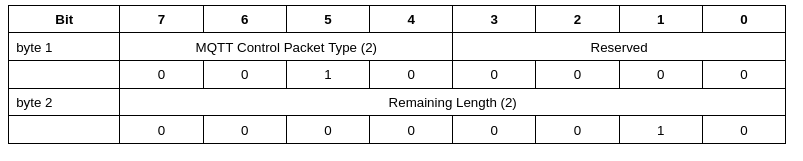
\includegraphics[width=\textwidth]{img/fixed_header_structure}
    \caption[Struktur des Fixed Headers in einem \gls{mqtt}-Paket]{Aus der Spezifikation von \gls{mqtt} Version 3.1.1~\cite{mqtt}
        zeigt die Struktur des Fixed Headers in einem \gls{mqtt}-Paket.
        Er besteht aus 2 Bytes und enthält den Steuerpakettyp (\textit{hier} 0010 für \texttt{CONNECT}) und Flags (hier \textit{Reserved})
        sowie die verbleibende Länge des Pakets.}
    \label{fig:fixed_header_structure}
\end{figure}
Der Fixed Header besteht aus drei Hauptbestandteilen~\ref{fig:fixed_header_structure}:
\begin{itemize}
    \item Steuerpakettyp: (4 Bits): MQTT definiert 14 Pakettypen (im Bereich von \texttt{0001} bis \texttt{1110}), was
    bedeutet, dass es 14 mögliche Werte für diese 4 Bits gibt
    \item Flags (4 Bits): Die Flags hängen vom Pakettyp ab, was die Anzahl der gültigen Kombinationen verringert
    \item Verbleibende Länge: Die verbleibende Länge gibt an, wie viele Bytes nach dem Fixed Header folgen
\end{itemize}
Die Spezifikation von \gls{mqtt} sieht vor, dass von den 14 möglichen Werten für den Steuerpakettyp nur 10 gültige Werte
für einen validen Steuerpakettypen existieren, die von dem Client zum Broker gesendet werden können~\cite{mqtt-fixed-header}.
Ausgegangen wird von der Generierung eines validen Connect Pakets, welches den Steuerpakettyp \texttt{CONNECT} hat.
Betrachtet wird zunächst die Wahrscheinlichkeit, dass der Fixed Header gültig ist.
Hierbei wird folgende Annahme getroffen:
\[
    P(\text{gültiger Fixed Header}) = P(\text{gültiger Steuerpakettyp}) \times P(\text{gültige Flags}) \times P(\text{gültige verbleibende Länge})
\]
Die Wahrscheinlichkeit, dass der Steuerpakettyp gültig ist, beträgt:
\[
    P(\text{gültiger Steuerpakettyp}) = \frac{M}{N} = \frac{1}{16}
\]
Wobei \textit{M} die Anzahl der gültigen Werte für den Steuerpakettyp \texttt{CONNECT} 0001 ist und \textit{N} die Anzahl der möglichen Werte, die
für die 4 Bits des Steuerpakettyps verwendet werden können.
Die Wahrscheinlichkeit, dass die Flags gültig sind, beträgt:
\[
    P(\text{gültige Flags}) = \frac{K}{N} = \frac{1}{16}
\]
Wobei \textit{K} die Anzahl der gültigen Kombinationen für die Flags ist und \textit{N} die Anzahl der möglichen Werte für die 4 Bits der Flags.
Hierbei ist zu beachten, dass die Flags bei einem \texttt{CONNECT}-Paket reserviert sind und somit nur die gültige Kombination
0000 für die Flags existieren.\newline
Das Zweite Byte des Fixed Headers enthält die verbleibende Länge des Pakets.
Die verbleibende Länge ist ein variable-length-integer, der die Anzahl der Bytes angibt, die nach dem Fixed Header folgen.
Sie kann Werte von 0 bis 127 annehmen.
Somit ergibt sich die Wahrscheinlichkeit, dass die verbleibende Länge gültig ist:
\[
    P(\text{gültige verbleibende Länge}) = \frac{128}{256}
\]
Die Wahrscheinlichkeit, dass der Fixed Header gültig ist, beträgt:
\[
    P(\text{gültiger Fixed Header}) = \frac{1}{16} \times \frac{1}{16} \times \frac{128}{256} \approx 1.938 \times 10^{-3}
\]
Der Variable Header enthält zusätzliche Informationen, die je nach Pakettyp variieren.
Für ein \texttt{CONNECT}-Paket enthält der Variable Header die Bytes für den Protokollnamen, die Protokollversion, Connect Flags
und Keep Alive.
Die Länge des Variable Headers beträgt 10 Bytes.
Die Wahrscheinlichkeit, dass der Variable Header gültig ist, beträgt:
\begin{multline}
    P(\text{gültiger Variable Header}) = P(\text{gültige Länge des Protokollnamens}) \\
    \times P(\text{gültiger Protokollnamen}) \times P(\text{gültige Protokollversion}) \times P(\text{gültige Connect Flags}) \\
    \times P(\text{gültiges Keep Alive})
\end{multline}
Die Länge des Protokollnamens ist festgelegt und beträgt 2 Bytes.
Die Wahrscheinlichkeit, dass die Länge des Protokollnamens gültig ist, beträgt:
\[
    P(\text{gültige Länge des Protokollnamens}) = \frac{1}{256} \times \frac{1}{256}
\]
\begin{figure}[H]
    \centering
    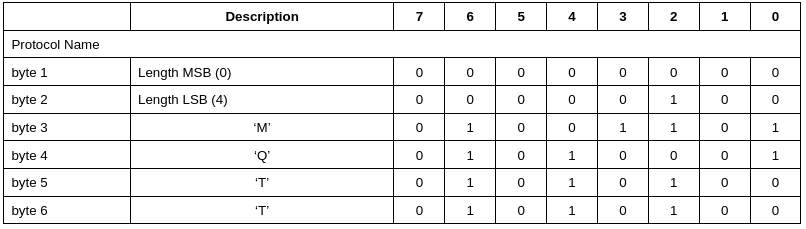
\includegraphics[width=\textwidth]{img/mqtt_prot_name}
    \caption[Struktur des Protokollnamens in einem \gls{mqtt}-Paket]{Zeigt die Struktur des Protokollnamens, entnommen aus der Spezifikation von \gls{mqtt} Version 3.1.1~\cite{mqtt-variable-header}.
        Der Protokollname ist festgelegt und muss \texttt{MQTT} sein und ist sechs Bytes lang.}
    \label{fig:mqtt_prot_name}
\end{figure}
Der Protokollname ist festgelegt auf vier Bytes und muss \texttt{MQTT} sein~\ref{fig:mqtt_prot_name}.
Aus der Struktur in der Abbildung~\ref{fig:mqtt_prot_name} ergibt sich die Wahrscheinlichkeit, dass der Protokollname gültig ist:
\[
    P(\text{gültiger Protokollname}) = \frac{1}{256}^4
\]
Zudem kommt hinzu, dass die Protokollversion festgelegt ist und \texttt{0x4} sein muss.
Die Protokollversion ist ein Byte lang und kann 256 mögliche Werte annehmen.
Somit ergibt sich die Wahrscheinlichkeit, dass die Protokollversion gültig ist:
\[
    P(\text{gültige Protokollversion}) = \frac{1}{256}
\]
Die Connect Flags sind ein Byte lang und können 256 mögliche Werte annehmen.
Die Wahrscheinlichkeit, dass die Connect Flags gültig sind, erschließt sich aus folgendem Regelwerk:
\begin{itemize}
    \item Bit 0 muss immer 0 sein
    \item Bit 1 kann 0 oder 1 sein. Wenn Bit 1 den Wert 0 hat, dann müssen die Bits 3-5 auch 0 sein
    \item Bit 2 kann 0 oder 1 sein
    \item Bit 3 und 4 können die Werte 00, 01 oder 10 annehmen, wenn Bit 1 den Wert 1 hat
    \item Bit 5 kann nur 1 sein, wenn Bit 1 den Wert 1 hat, ansonsten muss Bit 5 den Wert 0 besitzen
    \item Bit 6 und 7 können 0 oder 1 sein
\end{itemize}
Daraus ergibt sich die Wahrscheinlichkeit, dass die Connect Flags gültig sind:
\begin{equation}\label{eq:valid_connect_flags}
    P(\text{gültige Connect Flags}) = P(\text{Bit0}) \times P(\text{Bit1}) \times P(\text{Bit2}) \times P(\text{Bit3,4}) \times P(\text{Bit5}) \times P(\text{Bit6,7})
\end{equation}
\begin{itemize}
    \item Wenn Bit 2 = 0:

    \begin{itemize}
        \item Bit 3 + 4 = 00 (1 Möglichkeit)
        \item Bit 5 = 0 (1 Möglichkeit)
    \end{itemize}
\begin{multline}
    P(\text{Bit 3 + 4 + 5} \mid \text{Bit 2} = 0) = \frac{1}{8} \quad \\ \text{(es gibt 8 mögliche Kombinationen für Bit 3, 4 und 5, aber nur eine gültige)}
\end{multline}
    \item Wenn Bit 2 = 1:

    \begin{itemize}
        \item Bit 3 + 4 = 00, 01 oder 10 (3 Möglichkeiten)
        \item Bit 5 = 0 oder 1 (2 Möglichkeiten)
    \end{itemize}
\begin{multline}
    P(\text{Bit 3 + 4 + 5} \mid \text{Bit 2} = 1) = \frac{6}{8} \quad \\ \text{(es gibt 8 mögliche Kombinationen für Bit 3, 4 und 5, und 6 davon sind gültig)}
\end{multline}
\end{itemize}

\begin{multline}
    P(\text{Bit 3 + 4 + 5}) = P(\text{Bit 2} = 0) \times P(\text{Bit 3 + 4 + 5} \mid \text{Bit 2} = 0)+ P(\text{Bit 2} = 1) \times \\
    P(\text{Bit 3 + 4 + 5} \mid \text{Bit 2} = 1)
\end{multline}
\[
    P(\text{Bit 3 + 4 + 5}) = \frac{1}{2} \times \frac{1}{8}+ \frac{1}{2} \times \frac{6}{8}= \frac{1}{16}+ \frac{6}{16}= \frac{7}{16}
\]
Somit ergibt sich aus der Gleichung~\ref{eq:valid_connect_flags} die Wahrscheinlichkeit, dass die Connect Flags gültig sind:
\[
    P(\text{gültige Connect Flags}) = \frac{1}{2} \times 1 \times 1 \times \frac{7}{16} \times 1 \times 1 = \frac{7}{32}
\]
Das Keep Alive-Intervall ist ein 2-Byte-Wert, der die Zeit in Sekunden angibt, die der Client auf eine Antwort des Brokers
wartet.
Das Intervall kann Werte von 0 bis 65535 annehmen.
Die Wahrscheinlichkeit, dass das Keep Alive-Intervall gültig ist, beträgt 1, da alle Werte innerhalb der zwei Bytes zugelassen
werden.\newline
Die Wahrscheinlichkeiten für einen gültigen Variable Header sind somit:
\[
    P(\text{gültiger Variable Header}) = \left(\frac{1}{256}\right)^2 \times \left(\frac{1}{256}\right)^4 \times \frac{1}{256} \times \frac{7}{32} \times 1 \approx 3.036 \times 10^{-18}
\]
Um die Anzahl der Versuche zu berechnen, die notwendig sind, um mit einer 99-prozentigen Wahrscheinlichkeit ein gültiges
Paket mit korrekt generiertem Fixed und Variable Header zu erzeugen, wird folgende Formel verwendet:
\[
    n = \frac{\log(1 - P_{\text{Ziel}})}{\log(1 - P_{\text{Erfolg}})}
\]
Dabei beschreibt \textit{$P_{\textsubscript{Ziel}}$} die Zielwahrscheinlichkeit, dass ein gültiges Paket generiert wird, und
\textit{$P_{\textsubscript{Erfolg}}$} die Wahrscheinlichkeit, dass ein gültiger Fixed und Variable Header generiert wird.
Die Gesammtwahrscheinlichkeit für ein Paket mit einem gültigen Fixed und Variable Header beträgt:
\begin{multline}
    P(\text{Erfolg}) = P(\text{gültiger Fixed Header}) \times P(\text{gültiger Variable Header}) = \\
    1.938 \times 10^{-3} \times 3.036 \times 10^{-18} \\
    \approx 5.89 \times 10^{-21}
\end{multline}
Nun kann die Anzahl der Versuche berechnet werden, die notwendig sind, um mit einer 99-prozentigen Wahrscheinlichkeit ein
gültiges Paket zu generieren:
\[
    n = \frac{\log(1 - 0.99)}{\log(1 - 5.89 \times 10^{-21})} \approx 7.819 \times 10^{20}
\]
Bei einer gemessenen Ausführgeschwindigkeit von ca.\ 78 Paketen pro Sekunde würde es also ca. $10^{19}$ Sekunden dauern, um
mit einer Wahrscheinlichkeit von \SI{99}{\percent} ein gültiges Paket zu generieren.
Das entspricht ca.\ $3.22 \times 10^{11}$ Jahren für die Generierung eines korrekten Fixed und Variable Headers.\newline
Diese Berechnungen zeigen, dass das Fixieren von Teilen des Pakets (wie Fixed Header und Variable Header) die
Anzahl der benötigten Pakete zur Erzeugung eines gültigen Pakets erheblich reduziert.
Dies ist besonders wichtig für die Effizienz von Fuzzing-Tests, da es die Anzahl der Tests verringert, die benötigt werden,
um die gewünschten Ergebnisse zu erzielen.
\newline\newline
Durch das Fixieren bestimmter Schlüsselparameter des \gls{mqtt}-Pakets, wie dem Fixed Header und dem Topic, wird die Wahrscheinlichkeit,
dass ein gültiges Paket generiert wird, signifikant erhöht.
Dies ist besonders wichtig für effizientes Fuzzing, da es die Anzahl der möglichen ungültigen Pakete reduziert und die Effektivität der Tests steigert.
\begin{figure}[H]
    \centering
    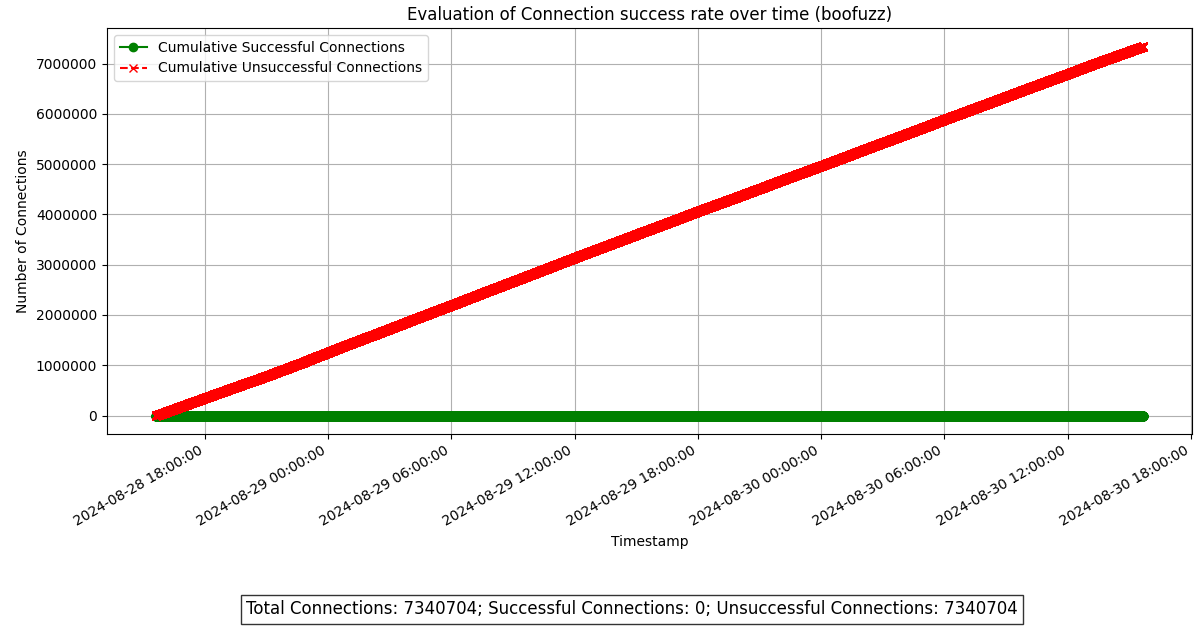
\includegraphics[width=\textwidth]{img/connection_evaluation_boofuzz}
    \caption{Vergleich der gültigen Pakete bei zufälligem Fuzzing mit boofuzz ohne statisch definierte Felder}
    \label{fig:valid_packets}
\end{figure}
\noindent Diese Grafik~\ref{fig:valid_packets} ist das Ergebnis einer Fuzzing-Kampagne, bei der über einen Zeitraum von 48 Stunden eine extrem hohe Anzahl an Verbindungsversuchen durchgeführt wurde.
Auch trotz der hohen Anzahl an Verbindungsversuchen, die in dieser Grafik dargestellt sind, konnte kein gültiges Paket generiert werden.
Das Fixieren der bereits genannten Felder führte bei einer weiteren Kampagne über 48 Stunden auch zu keinem gültigen Paket.
\begin{figure}[H]
    \centering
    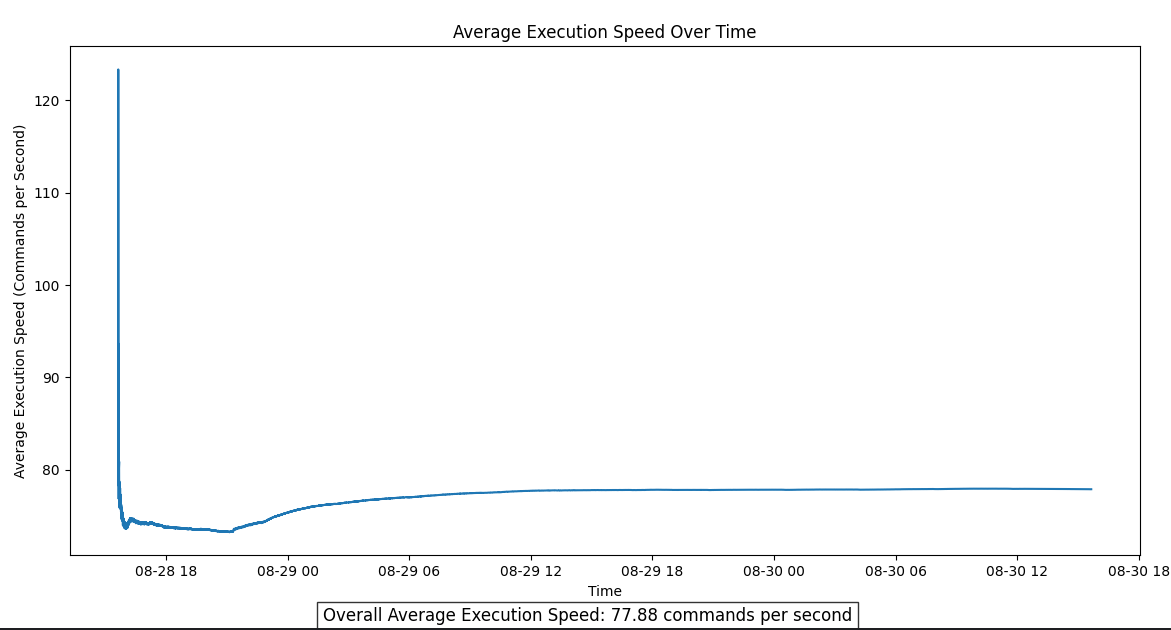
\includegraphics[width=\textwidth]{img/average_exec_speed_boofuzz_normal}
    \caption{Durchschnittliche Ausführungsgeschwindigkeit von boofuzz in einem Zeitraum von 48 Stunden}
    \label{fig:exec_speed_boo_normal}
\end{figure}
\noindent Die durchschnittliche Ausführungsgeschwindigkeit von boofuzz ist in dieser Grafik dargestellt.
In ihr ist zu erkennen, dass die Geschwindigkeit des Fuzzings über den Zeitraum von 48 Stunden relativ konstant bleibt.
Die einzige Ausnahme bildet der Anfangszeitraum der Fuzzing-Kampagne, in dem die Geschwindigkeit kurzzeitig rapide abfällt.
Dies hängt mit der Mutationsstrategie von boofuzz zusammen, die zu Beginn der Kampagne eine Vielzahl von großen Mutationen
durchführt, um das Zielsystem zu erkunden.
Zunächst wurden relativ kleine Pakete generiert, die jedoch aufgrund der geringen Wahrscheinlichkeit eines gültigen Pakets
keine Ergebnisse lieferten.
Im späteren Verlauf wurden jedoch größere Pakete generiert, was die Mutation erheblich verlangsamte.
Wichtig anzumerken ist die Strategie von boofuzz.
Trotz definition von statischen feldern im Header-Bereich wurden zufällige Bytes an den Kopf des Pakets angehängt.
Dies führte dazu, dass die Wahrscheinlichkeit eines gültigen Pakets weiterhin sehr gering war.
\begin{figure}[H]
    \centering
    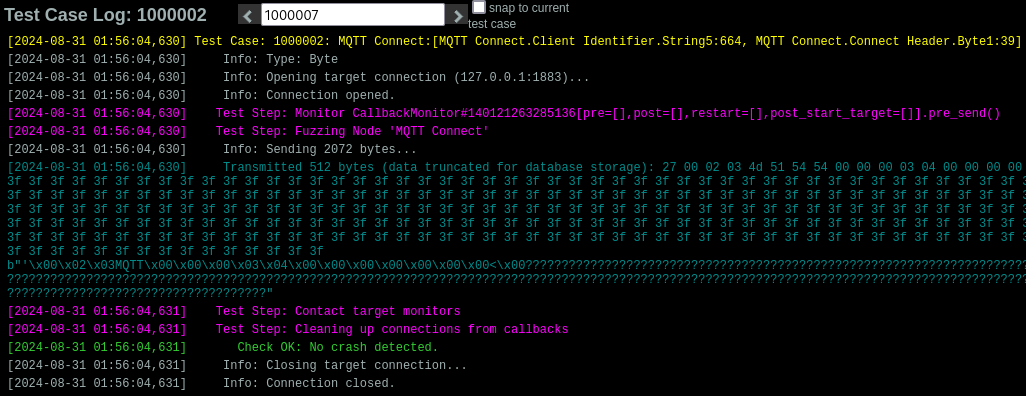
\includegraphics[width=\textwidth]{img/boofuzz_case_log}
    \caption{Diese Grafik zeigt einen Einblick zur Generierung von weiterhin ungültigen Paketen aufgrund des zufälligen Anhängens von Bytes
    im Header des Pakets.}
    \label{fig:boo_case_log}
\end{figure}
\noindent Erkennbar ist die Generierung falscher Pakete durch den festen definierten Header \texttt{0x020x03MQTT}, welcher aus der
Abbildung~\ref{fig:boo_case_log} hervorgeht.\newline\newline
Aus diesem Kapitel geht hervor, dass die Effektivität dieses Fuzzers stark von der Definition mehrerer Felder abhängt.
Im Falle von komplexeren Protokollen wie \gls{mqtt} ist es wichtig, dass eine Definition der Struktur der Felder in
der Implementierung des Fuzzers vonnöten ist, sodass die generierten Eingaben möglichst Effektiv sind.
Hierzu ist es wichtig, mehrere Aspekte des Protokolls zu definieren und zu fuzzen, um möglichst strukturiert und effektiv
an die Generierung von gültigen Paketen heranzugehen.
Dies kann in Zukunft dadurch umgesetzt werden, dass mehrere Instanzen des Fuzzers gestartet werden, die jeweils auf ein
bestimmtes Feld des \gls{mqtt}-Pakets fokussiert sind und somit die Wahrscheinlichkeit eines gültigen Pakets erhöht wird.
%! Author = chaorn
%! Date = 13.08.24

\subsection{Pulsar}\label{subsec:pulsar}
Im Folgenden werden alle Schritte zur Vorbereitung und Durchführung der Fuzzing Kampagne mit Pulsar beschrieben und
anschließend der daraus entstandene Erkenntnisgewinn geschlussfolgert.
\subsubsection{Setup}
Pulsar wurde mithilfe des von Pahl bereitgestellten Docker-Images~\cite{pulsar-docker} installiert.
Das Docker-Image wurde auf einem Ubuntu 20.04 LTS System installiert.
Weitere Abhängigkeiten, welche nicht in der Installation der Docker-Images enthalten sind, wurden manuell installiert und
in einer \texttt{requirements.txt} Datei festgehalten.
Für das Fuzzing mit Pulsar wird ein Netzwerkverkehr benötigt.
Dieser Netzwerkverkehr wird in Form von \gls{pcap}-Dateien gespeichert.
Hierfür wurde ein Python-Skript entwickelt, welches \gls{mqtt} spezifische Nachrichten an den Broker sendet und möglichst
viele Zustände vom Broker erreicht.
Die Nachrichten werden mithilfe des Tools \texttt{tcpdump} aufgezeichnet und in \gls{pcap}-Dateien abgelegt.
Die \gls{pcap}-Dateien werden in einem Ordner \textit{traffic} abgelegt.
Für den Start werden zusätzlich die \gls{pcap}-Dateien im Ordner \textit{traffic} über ein live-volume in den
Docker-Container eingehängt.
Alle gesammelten pcap-Dateien dienen für den weiteren Verlauf der Untersuchung.
Pulsar verwendet die \gls{pcap}-Dateien, um die State Machine zu erlernen.\newline\newline
Die Daten wurden in Kombination eines Python-Skripts, der Fuzzing Kampagne mit \gls{afl}Net und dem Tool
\texttt{tcpdump} gesammelt.
Das Python-Skript~\cite{python-script-input-generation} und \gls{afl}Net~\cite{aflnet-capture-traffic} wurden im Falle der Vorbereitung
auf die Fuzzing Kampagne mit Pulsar als Input-Generatoren verwendet.
Mithilfe dieser Tools wurde der Netzwerkverkehr aufgezeichnet und in \gls{pcap}-Dateien abgelegt.
Die \gls{pcap}-Dateien wurden in den Docker-Container mithilfe eines live-volumes eingehängt und Pulsar wurde gestartet~\cite{run-pulsar}.
Die gesammelten Daten wurden dann von Pulsar als Trainingsdaten verwendet, um das zu analysierende Protokoll zu erlernen.
\subsubsection{Erkenntnisgewinn}
Die Erkenntnisse des Fuzzing Kampagne mit Pulsar belaufen sich dabei auf die Art und Weise, wie Pulsar
den Netzwerkverkehr analysiert und das Protokoll erlernt.
Bei der Generierung von Input mit \gls{afl}Net und dem Python-Skript wurde darauf geachtet, dass möglichst viele Zustände
erreicht werden.
Jedoch wurde bei der Analyse des Netzwerkverkehrs festgestellt, dass Pulsar nicht in der Lage war, die State Machine
des \gls{mqtt} Protokolls korrekt zu erlernen.
Die Ursache hierfür ist, dass Pulsar die Startsequenz des Protokolls nicht korrekt erlernen konnte.
Durch das Generieren von Input mit \gls{afl}Net wurden viele falsche Pakete generiert, welche auch häufiger auftraten.
Mit unter ist das der Fall gewesen, dass Pulsar eine oft vorkommende Sequenz von vielen \textit{A}s als Startsequenz
des Protokolls interpretiert hat.
Diese Sequenzen sollten einen Fehlerzustand im Protokoll darstellen und nicht als Startsequenz interpretiert werden.
Da jedoch viele Implementierungen von Fehlerbehebungen in der State Machine des Protokolls vorhanden sind, wurde von
\gls{afl}Net auch eine Vielzahl von Fehlerzuständen generiert.
Dies liegt an der Art, wie \gls{afl}Net geeignete eingaben bewertet.
Eine Eingabe, die von \gls{afl}Net als geeignet bewertet wird, wird auch häufiger generiert.
Diese geeigneten Eingaben werden als geeignet bewertet, wenn sie viele Zustände erreichen.
Da jedoch viele Fehlerzustände in der State Machine des Protokolls vorhanden sind, werden auch viele Fehlerzustände
generiert.
Die vorhergehenden Versuche eines Verbindungsaufbaus mit einer Connect-Nachricht wurden nicht als Startsequenz
interpretiert.
Dies hatte zur Folge, dass im Zeitrahmen dieser Arbeit Pulsar nicht effektiv zum Laufen gebracht werden konnte.
Pulsar benötigt nämlich viel Zeit eine Markov-Kette zu erlernen und die State Machine zu approximieren, wenn besonders
viel Netzwerkverkehr aufgezeichnet wurde.
Im Rahmen dieser Arbeit wurden bis zu 7 Gigabyte an Netzwerkverkehr aufgezeichnet und Pulsar benötigte mehrere (ca.\ 35)
Stunden, um die State Machine zu erlernen.\newline\newline
Eine weitere Erkenntnis ist -- aufgrund der Geschwindigkeit des Lernprozesses -- dass Pulsar noch keine Hardwarebeschleunigung
mit bspw.\ einer \gls{gpu} unterstützt.
Die Hardwarebeschleunigung würde den Lernprozess beschleunigen und somit auch die State Machine schneller erlernen.
%! Author = chaorn
%! Date = 01.09.24
\subsection{Vergleich der erhobenen Metriken}\label{subsec:vergleich-der-erhobenen-metriken}
In diesem Kapitel werden die erhobenen Metriken der Fuzzer \gls{afl}Net, Pulsar und boofuzz miteinander verglichen.
Die Metriken wurden anhand der Anzahl der generierten Eingaben pro Sekunde und der Anzahl der reproduzierten Bugs gemessen.\newline\newline
Bei der Reinen Betrachtung der Anzahl der gesendeten Eingaben pro Sekunde ist Pulsar der langsamste Fuzzer.
Aufgrund der Implementierung des Fuzzers ist es ohne selbst geschriebene Skripte nicht möglich, die von Pulsar generierten
Eingaben zu automatisiert an das zu testende Programm zu senden.
Die Anzahl der generierten Eingaben pro Sekunde, die an das \gls{zup} gesendet werden, ist somit vom Tester abhängig.
Die Frage der Automatisierung stellt sich hierbei als entscheidend heraus, da die manuelle Eingabe von Eingaben in das
\gls{zup} die Geschwindigkeit des Fuzzers erheblich beeinflusst.
Der dadurch einhergehende Mangel von Automatisierung führt dazu, dass ein weiteres Monitoring des \gls{zup} notwendig ist,
um die generierten Eingaben und den Zustand des \gls{zup} zu überwachen.\newline
Der nächst schnellere Fuzzer ist \gls{afl}Net mit durchschnittlich 8 Ausführungen pro Sekunde.
Bei der Ausführungsgeschwindigkeit von \gls{afl}Net ist zu beachten, dass der Fuzzer aufgrund der Fuzzing-Strategie
in Kombination des bereits integrierten Monitoring des \gls{zup} etwas langsamer ist.
Die Geschwindigkeit des Fuzzers ist jedoch ausreichend, um eine Vielzahl von Eingaben zu generieren und an das \gls{zup}
zu senden.
Außerdem anzumerken ist, dass \gls{afl}Net das \gls{zup} immer wieder erneut startet.
Das hat zur Folge, dass alle Zustände des \gls{zup} immer wieder zurückgesetzt werden und somit die Initialisierung des
Programms immer wieder erneut durchgeführt werden muss.
Eine Möglichkeit, um das Fuzzing-Verhalten zu beschleunigen, wäre einen Fuzzing-Harness für das Programm zu schreiben, welcher es
ermöglichen würde den \textit{persistent mode} von \gls{afl} zu verwenden.
Mit ihm ist es möglich einen Zustand des \gls{zup} statisch zu implementieren, welcher dem des Programms nach dem
Initialisieren des \gls{zup} entspricht.
Diese Technik ist jedoch sehr aufwändig und benötigt sehr umfangreiches Wissen über die Funktionsweise des \gls{zup},
welches nur durch Sourcecodeanalyse oder Reverse Engineering des bereits kompilierten Programms möglich ist.
Dieser Fuzzing-Harnes kann unter umständen dazu führen, dass wichtige Programmpfade und Kontrollflüsse des \gls{zup}
vernachlässigt oder weggelassen werden können und die Wahrscheinlichkeit von false positives erhöht.\newline
Der schnellste Fuzzer ist boofuzz mit durchschnittlich 77,88 Ausführungen pro Sekunde.
Diese Anzahl von Ausführungen pro Sekunde ist auf die Implementierung des Fuzzers zurückzuführen.
Boofuzz gehört zu der gattung der Batch-Mutation-Fuzzer und generiert eine Vielzahl von Eingaben auf einmal.
Mithlife dieser Technik ist es möglich, eine Vielzahl von Eingaben zu generieren, welche jedoch nach Analyse der gesammelten
Logs nach simplen Brute-Force angriffen aussehen.\newline\newline
Die Anzahl der Ausführungen pro Sekunde ist jedoch nicht ausschlaggebend für die Effektivität eines Fuzzers.
Sie wird anhand der Anzahl der gefundenen Bugs pro Zeit gemessen.
Die Anzahl der gefundenen Bugs beläuft sich bei \gls{afl}Net auf 3 Bugs, bei Pulsar und boofuzz auf keinen einzigen.
Trotz einer niedrigen Anzahl an Ausführungen pro Sekunde konnte \gls{afl}Net bereits in sieben Minuten (vgl.\ Abb.~\ref{fig:aflnet_bugs})
den ersten Bug finden.
Dies spricht für eine hohe Effektivität des Fuzzing-Ansatzes von code-coverage und der Fuzzing-Strategie von \gls{afl}Net.
Die Zunahme der Präzision von generierten validen Paketen spiegelt sich ebenso in der Grafik~\ref{fig:mqtt-aflnet_stdout}
wider.\newline\newline
Zusammenfassend ist in Hinsicht der Forschungsfrage \textit{Q1} (siehe~\ref{researc-questions}) festzustellen, dass
\gls{afl}Net im Rahmen der vollzogenen Experimente der effektivste Fuzzer ist.
Die Anzahl der gefundenen Bugs und die Effizienz der generierten Eingaben sprechen für eine hohe Effektivität des Fuzzers
im Gegensatz zu den anderen Fuzzern.
Im Hinblick auf die Ausführungsgeschwindigkeit ist boofuzz der schnellste Fuzzer, jedoch konnte er keine Bugs finden.
Stellt man beide Fuzzer einander gegenüber, so beläuft sich die Ausführungsgeschwindigkeit von \gls{afl}Net auf durchschnittlich
8 Ausführungen pro Sekunde (siehe Abb.~\ref{fig:aflnet_execs}), während boofuzz auf durchschnittlich 77,88 Ausführungen pro
Sekunde (siehe Abb.~\ref{fig:exec_speed_boo_normal}) kommt.\newline
Auch in der Hinsicht der Effizienz der generierten Eingaben ist \gls{afl}Net der effizienteste Fuzzer.
Die generierten Eingaben sind präzise und enthalten mit zunehmender Zeit der Kampagne weniger ungültige Eingaben (siehe Abb.~\ref{fig:mqtt-aflnet_stdout}).
Dies ist jedoch nicht der Fall bei boofuzz, welcher eine Vielzahl von Eingaben generiert, die nach Brute-Force-Angriffen
aussehen und direkt beim Empfangen von dem \gls{mqtt}-Broker verworfen werden~\ref{fig:boo_case_log}.\newline
Zu dem Fuzzer Pulsar konnten jedoch keine aufschlussreichen Ergebnisse erzielt werden.